\chapter{MD StepEdit Page:}

The Step Edit page is used to program MCL's internal sequencer for a selected MD track. 
\screenshot{step.png}

\textit{To enter the MD Step Edit Page: First select desired track on the MD \textbf{[Function + Track N]}. Then press \textbf{[PageSelect + Trigger 5]} to open the StepEdit page.}

%\fbox{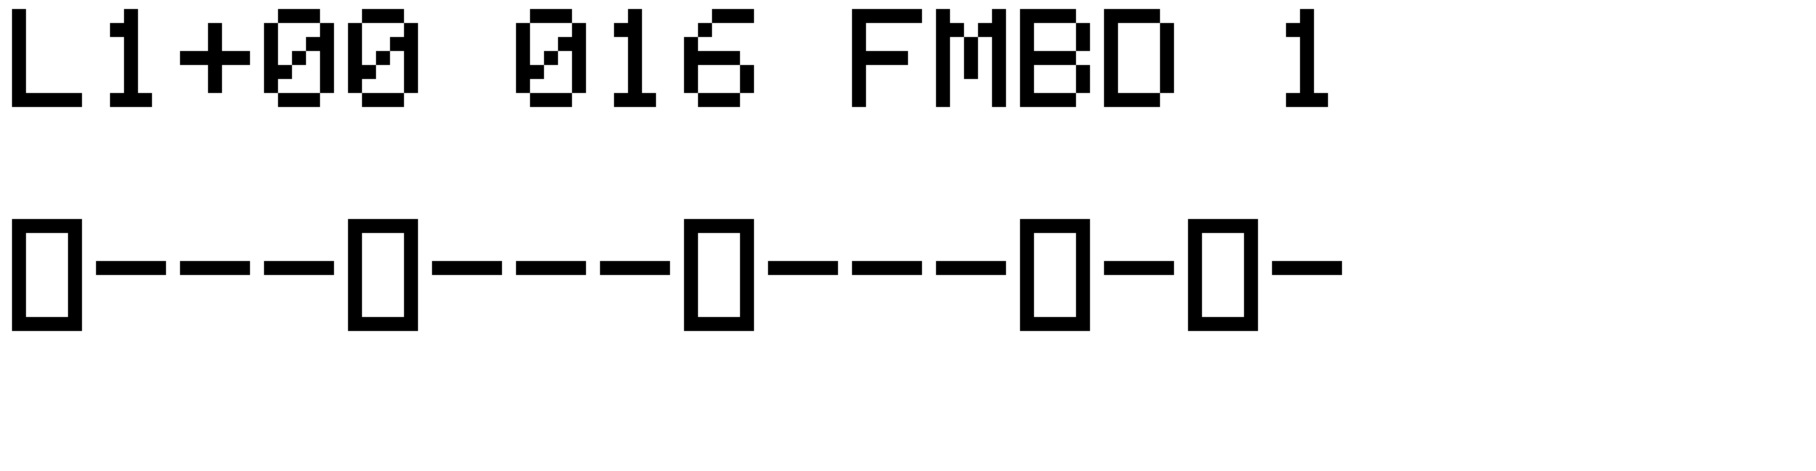
\includegraphics[scale=.40]{seq_step_page.png}}
\screenshot{step_action.png}

\encodersbuttons{Trig Condition}{Micro-Timing}{Track Length}{Note}{Toggles MD/Ext}{PageSelect}{Rotate View}{Track/Trig Menu}

\section{GUI:}
\begin{itemize}
\item The Step Edit Page uses the TI. The trigger buttons on the MD correspond to the 16 steps on the current page of the current track.
\item The 16 steps are displayed on the bottom row
\item Trig Conditions and Micro-Timing settings are per step and are chosen from encoders 1 and 2 respectively.
\end{itemize}

\section{Trig Conditions:}
\begin{itemize}
\item L1,L2,L3,L4,L5,L6,L7,L8 (For Ln, step is only triggered after every n iterations of track)
\item P10, P25, P50, P75, P90 (For Pxx, step has a xx percent chance of being triggered)
\item 1S. (One Shot trig, step is only triggered once)
\item Each trig condition above has a twin denoted by the \^{} character e.g L1\^{}, L2\^{}, P1\^{}. When these condition modes are selected, parameter locks and slides must also obey the trig condition.
\end{itemize}
\section{Micro Timing:}
\screenshot{utiming1.png}

\vspace{-0.3cm}

\section{Track Speed:}
All sequencer tracks can be played at various speeds. 1x, 2x, 3/2x, 3/4x, 1/2x, 1/4x, 1/8x. Triplets can be achieved using either 3/2x, 3/4x. 
Track speed can be adjusted from the Track Menu as explained in the previous chapter.

\section{Program a sequence:}
\begin{itemize}
\item Press and hold trigger button(s) on the MD to place triggers in the sequence.
\item Rotate encoders 1 and 2 to change the conditional mode or micro-timing if desired.
\end{itemize}

\section{Change Edit Mode:}
By default, the Step Edit page opens in Trig Edit mode. It is possible to change this edit mode to program the track's sequencer data for either Trigs, Locks, Slides or Mutes.
\begin{itemize}
\item To change the Edit mode, press and hold the\textbf{ [ Shift2 ]} to open the track menu, rotate \textbf{[ Encoder 2 ]} to the entry \textbf{Edit:}, then rotate \textbf{[ Encoder1 ]} to select either \textbf{"Trig, Lock, Slide or Mute"}.
\end{itemize}
\vspace{-0.3cm}

\section{Clearing a sequence:}
\begin{itemize}
\item To clear the current track, press and hold the\textbf{ [ Shift2 ]} to open the track menu, rotate \textbf{[ Encoder2 ]} to the entry \textbf{CLEAR}, then rotate \textbf{[ Encoder1 ]} to select \textbf{TRK}.
\item To clear all MD tracks, select \textbf{ALL}
\end{itemize}

\vspace{-0.3cm}

\section{Rotating visible sequence:}
Each track consists of 4 pages of 16 steps, for a total of 64 steps per track.
\begin{itemize}
\item Rotate the current track-page by pressing the \textbf{[ Load ] }button.
\item The MD's \textbf{[ Scale ]} button can also be used to rotate the sequence.
\end{itemize}

\vspace{-0.3cm}

\section{Changing track length:}
\begin{itemize}
\item Track length is controlled by rotating \textbf{[ Encoder 3 ]}. Only steps less than the current track length are drawn.
\item To change the lengths of all 16 tracks simultaneously hold down \textbf{[ Load ]} whilst rotating \textbf{[ Encoder 3 ]}.
\item Track length can also be set by holding \textbf{[ Load ]} and then selecting the corresponding step from the MD trigger interface. The track length is offset by the current track-page.
\end{itemize}

\section{Chromatic Step Edit:}
The Step Edit allows you to adjust a step's pitch by setting a note value. 
\begin{itemize}
\item Press and hold trigger button(s) on the MD. Rotating \textbf{[ Encoder 4 ]} will allow you change the note value of the selected steps.
\item A keyboard will be drawn on the display, showing the current note.
\end{itemize}
\screenshot{step_keyboard.png}

\section{Parameter Locks:}
The Step Edit page now allows you to enter parameter locks directly from the MD. Simply select a trigger button and rotate the corresponding parameter on the MD. Up to four parameter types can be locked on any given track. See the Sequencer Parameter Locks pages more details.
\newpage
\section{Trig Preview:}
Hold down the desired trigger and press \textbf{[ Enter ]} on the Machinedrum.
\section{Slides:}
Each parameter lock can be made to slide up or down to the nearest step containing a parameter lock of the same type.
\\\\
To add slides to your sequence change the Edit Mode to "SLIDE" (see above).
\section{Mutes:}
Individual steps of your sequence can be muted, by placing a mute trig at the corresponding position. Mutes are reset on sequencer restart.\\\\ 
To add mutes to your sequence change the Edit Mode to "MUTE" (see above).
\section{Shift Sequence:}
The sequence of an individual track can be shifted left of right. Press \textbf{[ Function ]} + \textbf{[ Left ]} or \textbf{[ Right ]} on the MD. The sequencer menu can also be used to shift the entire pattern via the SHIFT option.
Similarly you can reverse a track's sequence from the sequencer menu option REVERSE.
\section{Step Menu:}

\screenshot{step_menu.png}
The step menu will be opened by selecting one or more step/trig from the TI and when holding \textbf{[Shift 2]}. The entry activated on release, similar to the slot menu.
The step menu consists of the following entries:

\begin{figure}[hb]
    \begin{tabular}{|l|l|}
    \hline
    \rowcolor[HTML]{C0C0C0} 
    Entry            & Function \\ \hline
    Clear            & Locks: Clear step's parameter locks \\ \hline
    Copy         & Copy step\\ \hline
    Paste        & Paste step\\ \hline
    Mute         & Mute or Unmute step\\ \hline
    \end{tabular}
\end{figure}